\documentclass[12pt,a4paper,oneside]{article}

\usepackage[utf8]{inputenc}
\usepackage[portuguese]{babel}
\usepackage[T1]{fontenc}
\usepackage{amsmath}
\usepackage{amsfonts}
\usepackage{amssymb}
\usepackage{graphicx}

\usepackage{xcolor}
% Definindo novas cores
\definecolor{verde}{rgb}{0.25,0.5,0.35}
\definecolor{jpurple}{rgb}{0.5,0,0.35}
% Configurando layout para mostrar codigos Java
\usepackage{listings}
\lstset{
  language=Java,
  basicstyle=\ttfamily\small, 
  keywordstyle=\color{jpurple}\bfseries,
  stringstyle=\color{red},
  commentstyle=\color{verde},
  morecomment=[s][\color{blue}]{/**}{*/},
  extendedchars=true, 
  showspaces=false, 
  showstringspaces=false, 
  numbers=left,
  numberstyle=\tiny,
  breaklines=true, 
  backgroundcolor=\color{cyan!10}, 
  breakautoindent=true, 
  captionpos=b,
  xleftmargin=0pt,
  tabsize=4,
  escapeinside=||
}

\author{\\Universidade Federal de Goiás (UFG) - Regional Jataí\\Bacharelado em Ciência da Computação \\Física para Ciência da Computação \\Esdras Lins Bispo Jr.}

\title{\sc \huge Primeiro Teste}

\date{11 de outubro de 2016}

\begin{document}

\maketitle

{\bf ORIENTAÇÕES PARA A RESOLUÇÃO}

\footnotesize

\begin{itemize}
	\item A avaliação é individual, sem consulta;
	\item A pontuação máxima desta avaliação é 10,0 (dez) pontos, sendo uma das 05 (cinco) componentes que formarão a média final da disciplina: dois testes, duas provas e exercícios-bônus;
	\item A média final ($MF$) será calculada assim como se segue
	\begin{eqnarray}
		MF & = & MIN(10, S) \nonumber \\
		S & = & (\sum_{i=1}^{4} 0,2.T_i ) + 0,2.P  + EB \nonumber
	\end{eqnarray}
	em que 
	\begin{itemize}
		\item $S$ é o somatório da pontuação de todas as avaliações,
		\item $T_i$ é a pontuação obtida no teste $i$,
		\item $P$ é a pontuação obtida na prova, e
		\item $EB$ é a pontuação total dos exercícios-bônus.
	\end{itemize}
	\item O conteúdo exigido compreende os seguintes pontos apresentados no Plano de Ensino da disciplina: (1) Fundamentos Matemáticos e (2) Medidas Físicas e Vetores.
\end{itemize}


\begin{center}
	\fbox{\large Nome: \hspace{10cm}}
	\fbox{\large Assinatura: \hspace{9cm}}
\end{center}

\newpage

\normalsize

\begin{enumerate}

	\item (5,0 pt) {\bf (Halliday 1.15)} Três relógios digitais, A, B e C, funcionam com velocidades diferentes e não têm leituras simultâneas de zero. A Figura 1 mostra leituras simultâneas de pares dos relógios em quatro ocasiões. (Na primeira ocasião, por exemplo, B indica 25,0 s e C indica 92,0 s.) Se o intervalo entre dois eventos é 600 s de acordo com o relógio A, qual é o intervalo entre os eventos 
		\begin{enumerate}
			\item no relógio B, e
			\item no relógio C?
		\end{enumerate}
	Verifique também se
		\begin{enumerate}
			\setcounter{enumii}{2}
			\item Quando o relógio A indica 400 s, qual é a indicação do relógio B?
			\item Quando o relógio C indica 15,0 s, qual é a indicação do relógio B?
		\end{enumerate}
	(Suponha que as leituras sejam negativas para instantes anteriores a zero.)
	
	\begin{center}
		\begin{figure}[htb]
			\centering		
			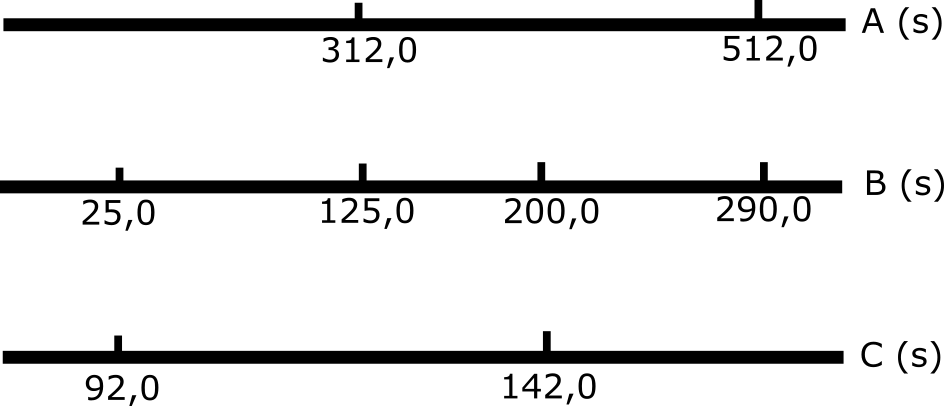
\includegraphics[scale=0.4]{images/hal13.png}
			\caption{Leitura simultânea de pares de relógios em quatro ocasiões (relógios A, B e C).}
		\end{figure}
	\end{center}
	
	\item (5,0 pt) Em JavaScript, crie um protótipo de objeto {\tt Particula} que tenha as propriedades (i) {\tt nome}, (ii) {\tt carga}, (iii) {\tt spin}, e (iv) {\tt descricao}. O {\tt nome} é uma cadeia; a {\tt carga} e o {\tt spin} são valores numéricos; e a {\tt descricao} é uma função que exibe, via {\tt console.log}, todas as demais propriedades de {\tt Particula}. Crie um objeto a partir de {\tt Particula}. Atribua valores para as propriedades ao seu gosto.
	
	\end{enumerate}
\end{document}